\documentclass[letterpaper, 12pt]{article} 
\usepackage{amsmath}
\usepackage{bm}
\usepackage{graphicx}
\usepackage{amsfonts}
\usepackage{fancyhdr}
\usepackage{color}
\setlength{\parindent}{0pt
}\pagestyle{fancy}
\rhead{Roland Gee 995293711}
\title{Assignment 1}
\author{Roland Gee 995293711}
\begin{document}

\maketitle

\section*{Logistic Regression}
\begin{itemize}
	\item[1.1]
		Baye's Rule : \\

		$p(y=1 | x) = \frac{p(x|y = 1)p(y=1)}{p(x|y = 0)p(y = 0) + p(x|y = 1)p(y = 1)}$ \\

		We know the following: \\

		\begin{itemize}
			\item[1.] $y$ follows a Bernoulli distribution
			\item[2.]  Each $x_i$ is follows Gaussian distribution with class means $\mu_{i0} \mu_{i1}$ and shared class std $\\sigma_i$
			\item[3.] Dimensions of $\bm{x}$ are conditionally independent with y
		\end{itemize}

		Simplifying the above equation \\

		$p(y=1 | x) = \frac{1}{1 + \frac{p(y=0)p(x|y = 0)}{p(y = 1)p(x|y = 1)}}$ \\		

		$= \frac{1}{1 + exp(ln\frac{p(y=0)p(x|y = 0)}{p(y = 1)p(x|y = 1)})}$

		Because of 3. , $p(x|y = 1) = \prod_i^D p(x_i|y = 1)$ and $p(x|y = 0) = \prod_i^D p(x_i|y = 0)$. Also using the fact that ln($ab$) = ln(a) + ln(b), we can simplify the above to the following: \\

		$= \frac{1}{1 + exp(ln\frac{p(y=0)}{p(y=1)} + \sigma_i^D ln\frac{p(x_i|y = 0)}{p(x_i|y = 1)})}$

		From 1. , $p(y = 1) = \alpha$ and $p(y = 0) = 1 - \alpha$: \\

		$= \frac{1}{1 + exp(ln\frac{\alpha}{1 - \alpha} + \sum_i^D ln\frac{p(x_i|y = 0)}{p(x_i|y = 1)})}$ \\

		From 2, $p(x_i|y=0) = \frac{1}{\sqrt{2\pi\sigma_i^2}exp(\frac{-(x_i - \mu_{i0})^2}{2\sigma_i^2})}$, $p(x_i|y=1) = \frac{1}{\sqrt{2\pi\sigma_i^2}exp(\frac{-(x_i - \mu_{i1})^2}{2\sigma_i^2})}$

		Simplifying $\sum_i^D ln\frac{p(x_i|y = 0)}{p(x_i|y = 1)}$ \\

		$\sigma_i^D ln\frac{p(x_i|y = 0)}{p(x_i|y = 1)} = \sum_i^D\frac{\mu_{i0} - \mu_{i1}}{\sigma_i^2}x_i + \frac{\mu^2_{i1} - \mu^2_{i0}}{2\sigma^2_i}$ \\

		Substituting back in: \\

		$= \frac{1}{1 + exp(ln\frac{1 - \alpha}{\alpha} + \sum_i^D\frac{\mu_{i0} - \mu_{i1}}{\sigma_i^2}x_i + \frac{\mu^2_{i1} - \mu^2_{i0}}{2\sigma^2_i})}$ \\

		To make the equation equivalent to logistic regression, we do the following: \\

		let $-b = -ln\frac{1 - \alpha}{\alpha} - \sum_i^D \frac{-\mu^2_{i1} + \mu^2_{i0}}{2\sigma^2_i}$, $-w_i = -\frac{\mu_{i0} + \mu_{i1}}{\sigma_i^2}$ \\

		$= \frac{1}{1 + exp(-\sum_i^D w_ix_i - b)}$ \\ 



	\item[1.2]
		The definition of MLE for a binary output $y$ is the maximization of the following expression $L = \prod_{i=1}^N p(y = y_i | x)$. \\

		$p( y = y_i | x^n, w, b) = \sigma(w^Tx^{(n)} + b)(1 - \sigma(w^Tx^{(n)})$ \\

		$L = \prod_{i=1}^N [\sigma(w_i^Tx_i^{(n)}] + b)]^{1 - y_i}[(1 - \sigma(w_i^Tx_i^{(n)})]^{(y_i)}$ \\

		$\sigma(w_i^Tx_i^{(n)} + b) = \frac{1}{1 + \exp(-z)}$ where $z = \sum_i^D w_ix_i + b$ \\

		$\ln \sigma(w_i^Tx_i^{(n)}] + b) = -\ln (1 + \exp(-z))$ \\		

		$1 - \sigma(w_i^Tx_i^{(n)})]^{(y_i)} = \frac{\exp(-z)}{1 + \exp(-z)}$\\

		$\ln (1- \sigma(w_i^Tx_i^{(n)}] + b)) = -z - \ln(1 + \exp(-z))$ \\

		$-\ln L = -\sum_i^N (1-y) (-\ln (1 + \exp(-z))) + \sum_i^N y(-z - \ln(1 + \exp(-z)))$ \\

		$= -\sum_i^N -\ln (1 + \exp(-z)) + y(\ln (1 + \exp(-z))) + \sum_i^N -yz -y(\ln(1 + \exp(-z)))) $ \\

		$= \sum_i^N \ln (1 + \exp(-z)) + \sum_i^N yz)$ \\

		let $l = -\ln L$: \\

		$z = \sum_i^D w_ix_i + b$ \\

		To find $\frac{\delta l}{\delta w}$ , we have to derive $\frac{\delta l}{\delta w_j}$ where $w_j$ represents an individual weight in our model. \\

		With respect to $-z$, we only want to use the weight and corresponding input $i = j \in D$. Hence $\sum_i^D w_ix_i$ becomes $w_jx_j$ when calculating the derivative. \\

		$\frac{\delta l}{\delta w_j} = \sum_i^N \frac{\delta (\ln(1 + exp(-z)))}{\delta w_j} + \sum_i^N \frac{\delta y(z)}{\delta w_j}$ \\

		Applying product rules will give the following result: \\

		$\frac{\delta l}{\delta w_j} = \sum_i^N y_ix_j + \sum_i^N \frac{exp(-z_i)}{1 + exp(-z_i)}$ \\

		$\frac{\delta l}{\delta b} = \sum_i^N \frac{\delta (\ln(1 + exp(-z_i)))}{\delta b} + \sum_i^N \frac{\delta y(z_i)}{\delta b}$ \\

		$\frac{\delta l}{\delta b} = \sum_i^N -y_i - \sum_i^N \frac{exp(-z_i)}{1 + exp(-z_i)}$ 
	\item[1.3]
\end{itemize}
\section*{Digit Classification}
\begin{itemize}
	\item[2.1]
		Here is the following table and corresponding plot for kNN performance: \\
		\begin{center}
			\begin{tabular}{ l | r }
				k &rate\\
				\hline
				1 &0.82\\
				3 &0.86\\
				5 &0.86\\
				7 &0.86\\
				9 &0.84
			\end{tabular}
		\end{center}
		\begin{center}
			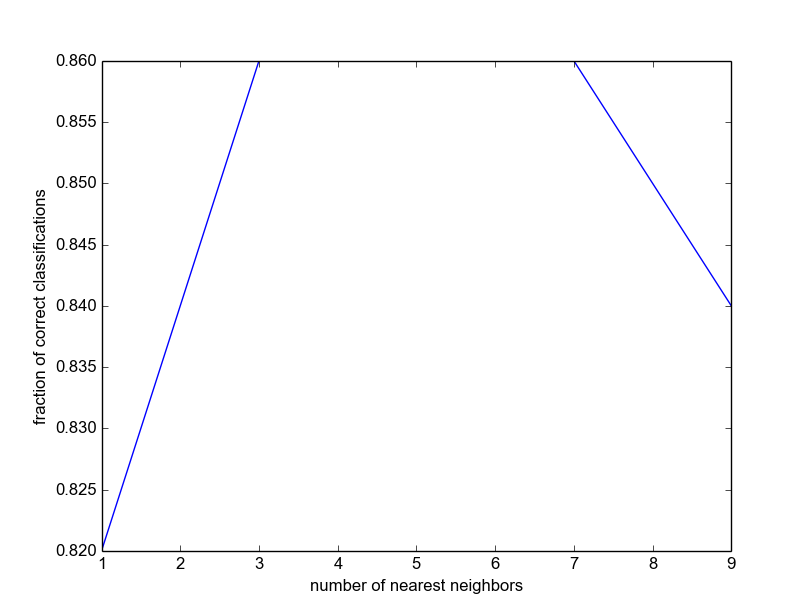
\includegraphics[scale=0.25]{figure_1.png}
		\end{center}

		The minimum $k$ that will produce the maximum $k*$ would be $k = 3$. Also since we are dealing with binary classification, $k$ should be odd. The rate for $k = 1$ is 0.82 and $k = 5$ is 0.86. The test performance in this case does correspond to the validation performance. Test performance is $O(dn)$. Validiation performance is $KO(\frac{dn}{K})$.

	\item[2.2]
		The best paramters that I have found were a learning rate of 0.05, with 150 iterations. On a small training set, LR overfits with training accuracy of 100, valid CE of 184, and valid accuracy of 88. On the regular training set, LR prefomed quite well with training accuracy with 83, valid CE of 185, and valid accuracy of 84. On the test set, training accuracy was 88, valid CE of 224, and valid accuracy of 90. \\

		Iterations vs CE Plot for small training set: \\
		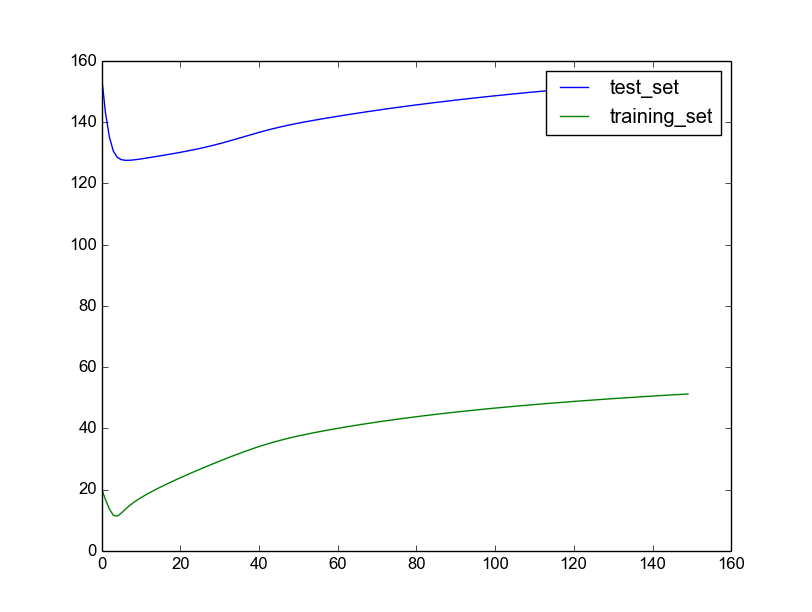
\includegraphics[scale = 0.50] {small_set.png} \\

		Iterations vs CE Plot for regular training set: \\
		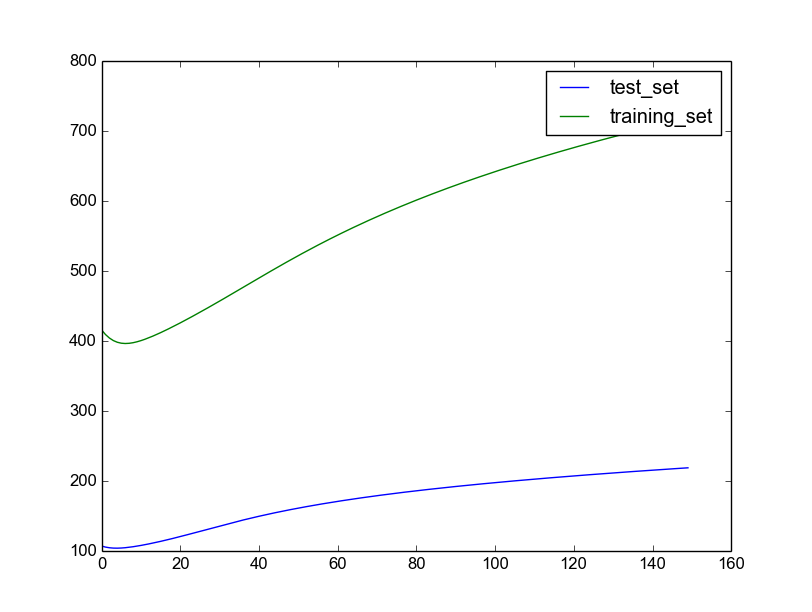
\includegraphics[scale = 0.50] {regular_set.png}
	\item[2.3]
	\newpage
	\item[2.4]
		Correctness fraction of Naive Bayes is 0.80. \\

		Mean/Var Scatterplot: \\

		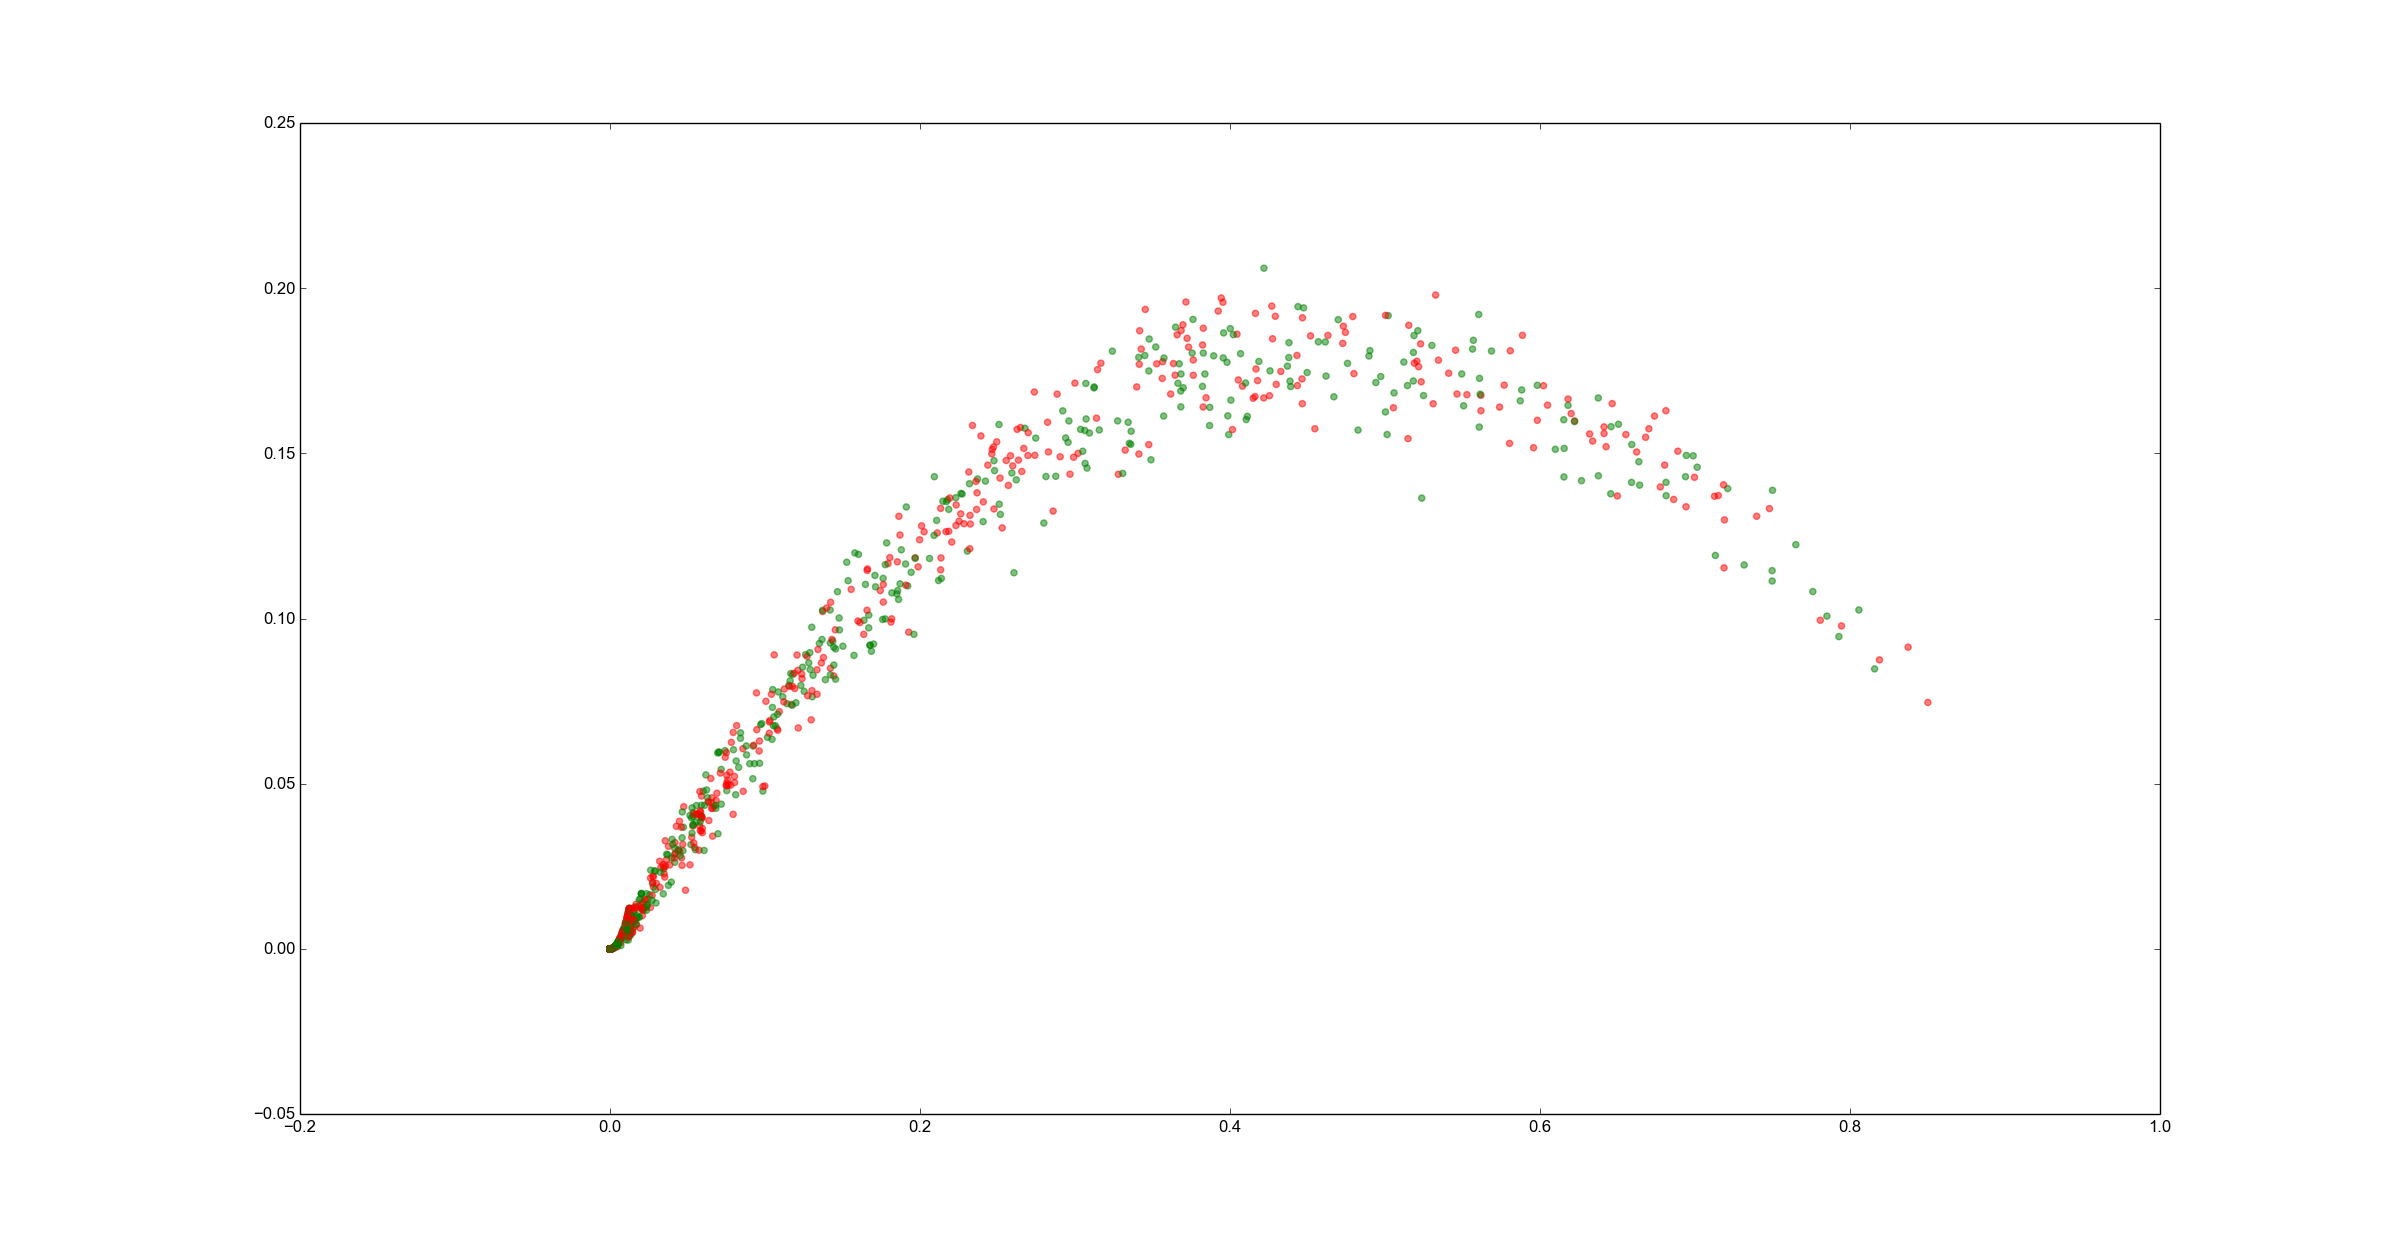
\includegraphics[scale=0.25]{mean_var_scatter.png}	
	\item[2.5]
		In terms of correctness, KNN and Naive Bayes fair the best with 0.82 and 0.80 success rate respectively whereas Logistic Regression  without L2 had a success rate of 0.76 (did not run with L2). \\

		In this case, Naive Bayes faired well because the assumptions of the conditonals being independent and Guassian were correct. However for datasets for which these assumptions do not hold, I would go with Logistic Regression. \\

		To briefly discuss the differences between these classifiers, Naive Bayes is considered to be a high bias/low variance classifier wheras KNN and Logistic Regression are considered to be low bias / high variance classifiers. 

		High variance can cause overfitting, which can be seen in smaller data sets. I experienced that when running Logistic Regression over the small training set with even with a moderate learning rate of 0.1. However because the problem with high variance can be combatted by increasing the size of the training set. This makes Logistic Regression and KNN good choices for large data sets due to their low bias.
		
		Bayes classifier on the other hand have its own advantages. It is not sensitive to irrelevant features (due to independence assumption) and it is very quick to train. So for situations where performance is important and the independence assumption can be made, Bayes is very useful.
\end{itemize}
\end{document}